\documentclass[10pt]{beamer}

% Idioma e codificação
\usepackage[brazil]{babel}
\usepackage[utf8]{inputenc}
\usepackage[T1]{fontenc}

% Temas e Cores
\usetheme{Madrid}
\definecolor{maincolor}{RGB}{0,100,50}
\usecolortheme[named=maincolor]{structure}

% Pacotes Extras
\usepackage{booktabs}
\usepackage{listings}
\usepackage{tikz}
\usetikzlibrary{shapes, arrows, positioning}

% Configuração de SQL
\lstset{
    language=SQL,
    basicstyle=\ttfamily\small,
    keywordstyle=\color{blue}\bfseries,
    commentstyle=\color{gray}\itshape,
    stringstyle=\color{red},
    frame=single,
    breaklines=true,
    showstringspaces=false
}

\title{SQL Joins: Conectando Dados}
\subtitle{Entendendo Relacionamentos em Banco de Dados}
\author{Me.~Sergio Souza Novak}
\date{\today}

\begin{document}

% Slide 1: Titulo
\begin{frame}
    \titlepage
\end{frame}

% Slide 2: O que é um JOIN?
\begin{frame}{O que é um JOIN?}
    \begin{itemize}
        \item SQL Joins são usados para combinar linhas de duas ou mais tabelas.
        \item A combinação é feita com base em uma \textbf{coluna comum} (geralmente Chave Primária e Chave Estrangeira).
        \item É a base de qualquer sistema relacional: as informações são separadas em entidades, mas unidas na consulta.
    \end{itemize}
\end{frame}

% Slide 3: Nossas Tabelas de Exemplo
\begin{frame}{Nossas Tabelas de Exemplo}
    \begin{columns}
        \begin{column}{0.45\textwidth}
            \textbf{Tabela: Alunos}
            \small
            \begin{table}
                \begin{tabular}{lcr}
                \toprule
                \textbf{id} & \textbf{nome} & \textbf{c\_id} \\ \midrule
                1 & Ana & 10 \\
                2 & João & 20 \\
                3 & \alert{Pedro} & \alert{30} \\ \bottomrule
                \end{tabular}
            \end{table}
        \end{column}
        \begin{column}{0.45\textwidth}
            \textbf{Tabela: Cursos}
            \small
            \begin{table}
                \begin{tabular}{lr}
                \toprule
                \textbf{id} & \textbf{nome\_curso} \\ \midrule
                10 & Engenharia \\
                20 & Direito \\
                \alert{40} & \alert{Medicina} \\ \bottomrule
                \end{tabular}
            \end{table}
        \end{column}
    \end{columns}
    \vspace{0.5em}
    \centering
    \footnotesize \textit{Obs: Pedro tem curso 30 (não existe). Medicina não tem alunos.}
\end{frame}

% Slide 4: Tipos de Joins
\begin{frame}{Tipos Principais de Joins}
    \begin{center}
    \begin{tikzpicture}[node distance=1.5cm]
        \node[ellipse, draw, fill=blue!10] (inner) {INNER JOIN};
        \node[ellipse, draw, fill=green!10, left=of inner] (left) {LEFT JOIN};
        \node[ellipse, draw, fill=red!10, right=of inner] (right) {RIGHT JOIN};
        \node[ellipse, draw, fill=yellow!10, below=of inner] (full) {FULL JOIN};
        \node[ellipse, draw, fill=gray!10, below=of full] (cross) {CROSS JOIN};
    \end{tikzpicture}
    \end{center}
\end{frame}

% Slide 5: INNER JOIN
\begin{frame}[fragile]{INNER JOIN (A interseção)}
    \begin{columns}
        \begin{column}{0.6\textwidth}
            Retorna apenas registros que possuem \textbf{correspondência em ambas} as tabelas.
            \begin{lstlisting}
SELECT A.nome, C.nome_curso
FROM Alunos AS A
INNER JOIN Cursos AS C ON A.curso_id = C.id;
            \end{lstlisting}
        \end{column}
        \begin{column}{0.35\textwidth}
            \centering
            \begin{tikzpicture}[scale=0.8]
                \draw (0,0) circle (1.2);
                \draw (1.2,0) circle (1.2);
                \begin{scope}
                    \clip (0,0) circle (1.2);
                    \fill[maincolor!60] (1.2,0) circle (1.2);
                \end{scope}
                \node at (-0.5,0) {\scriptsize \textbf{Alunos}};
                \node at (1.7,0) {\scriptsize \textbf{Cursos}};
            \end{tikzpicture}
        \end{column}
    \end{columns}
    \textbf{Resultado:}
    \small
    \begin{table}
        \begin{tabular}{ll}
        \toprule
        \textbf{nome} & \textbf{nome\_curso} \\ \midrule
        Ana & Engenharia \\
        João & Direito \\ \bottomrule
        \end{tabular}
    \end{table}
    \footnotesize \textit{* Pedro e Medicina ficaram de fora.}
\end{frame}

% Slide 6: LEFT JOIN
\begin{frame}[fragile]{LEFT JOIN (Prioridade à esquerda)}
    \begin{columns}
        \begin{column}{0.6\textwidth}
            Retorna \textbf{todos} da tabela da esquerda e os correspondentes da direita.
            \begin{lstlisting}
SELECT A.nome, C.nome_curso
FROM Alunos AS A
LEFT JOIN Cursos AS C ON A.curso_id = C.id;
            \end{lstlisting}
        \end{column}
        \begin{column}{0.35\textwidth}
            \centering
            \begin{tikzpicture}[scale=0.8]
                \fill[maincolor!60] (0,0) circle (1.2);
                \draw (0,0) circle (1.2);
                \draw (1.2,0) circle (1.2);
                \node at (-0.5,0) {\scriptsize \textbf{Alunos}};
                \node at (1.7,0) {\scriptsize \textbf{Cursos}};
            \end{tikzpicture}
        \end{column}
    \end{columns}
    \textbf{Resultado:}
    \small
    \begin{table}
        \begin{tabular}{ll}
        \toprule
        \textbf{nome} & \textbf{nome\_curso} \\ \midrule
        Ana & Engenharia \\
        João & Direito \\
        \alert{Pedro} & \alert{NULL} \\ \bottomrule
        \end{tabular}
    \end{table}
\end{frame}

% Slide 7: RIGHT JOIN
\begin{frame}[fragile]{RIGHT JOIN (Prioridade à direita)}
    \begin{columns}
        \begin{column}{0.6\textwidth}
            Retorna \textbf{todos} da tabela da direita e os correspondentes da esquerda.
            \begin{lstlisting}
SELECT A.nome, C.nome_curso
FROM Alunos AS A
RIGHT JOIN Cursos AS C ON A.curso_id = C.id;
            \end{lstlisting}
        \end{column}
        \begin{column}{0.35\textwidth}
            \centering
            \begin{tikzpicture}[scale=0.8]
                \fill[maincolor!60] (1.2,0) circle (1.2);
                \draw (0,0) circle (1.2);
                \draw (1.2,0) circle (1.2);
                \node at (-0.5,0) {\scriptsize \textbf{Alunos}};
                \node at (1.7,0) {\scriptsize \textbf{Cursos}};
            \end{tikzpicture}
        \end{column}
    \end{columns}
    \textbf{Resultado:}
    \small
    \begin{table}
        \begin{tabular}{ll}
        \toprule
        \textbf{nome} & \textbf{nome\_curso} \\ \midrule
        Ana & Engenharia \\
        João & Direito \\
        \alert{NULL} & \alert{Medicina} \\ \bottomrule
        \end{tabular}
    \end{table}
\end{frame}

% Slide Extra: Curiosidade sobre RIGHT JOIN
\begin{frame}{RIGHT JOIN: Implementação e Documentação}
    \begin{center}
        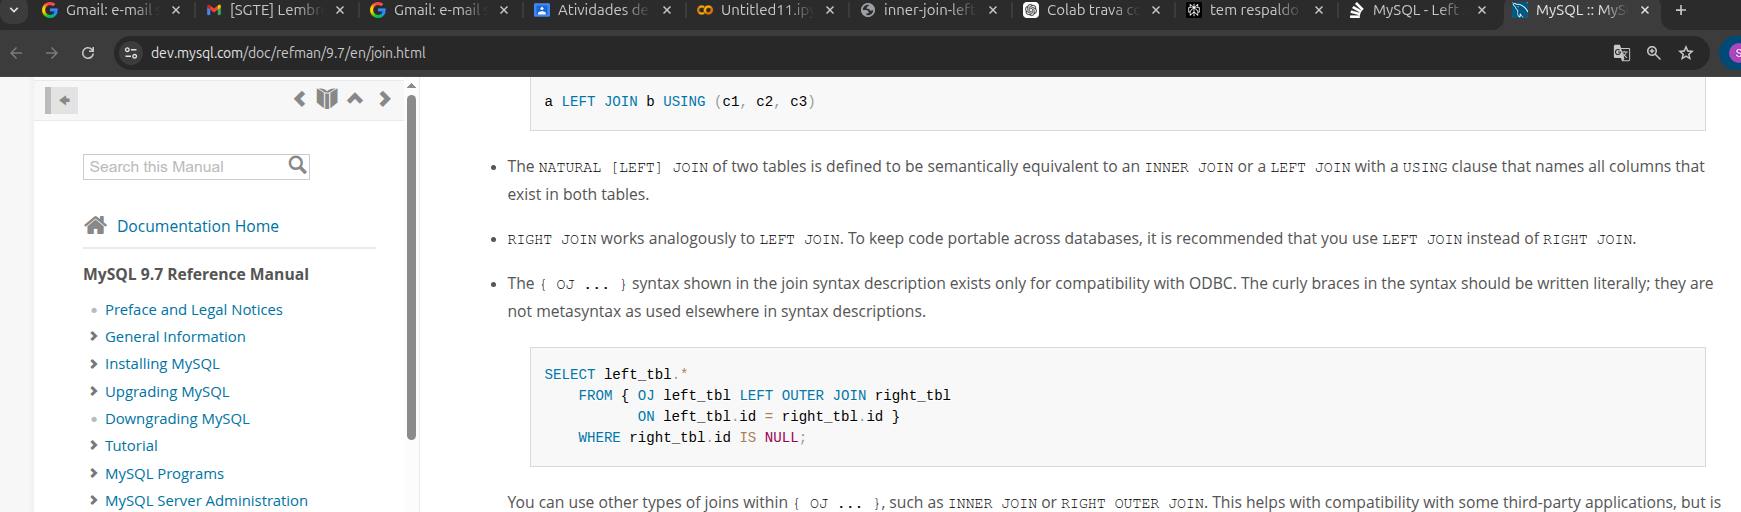
\includegraphics[width=0.45\textwidth]{mysql1.png}
        \hfill
        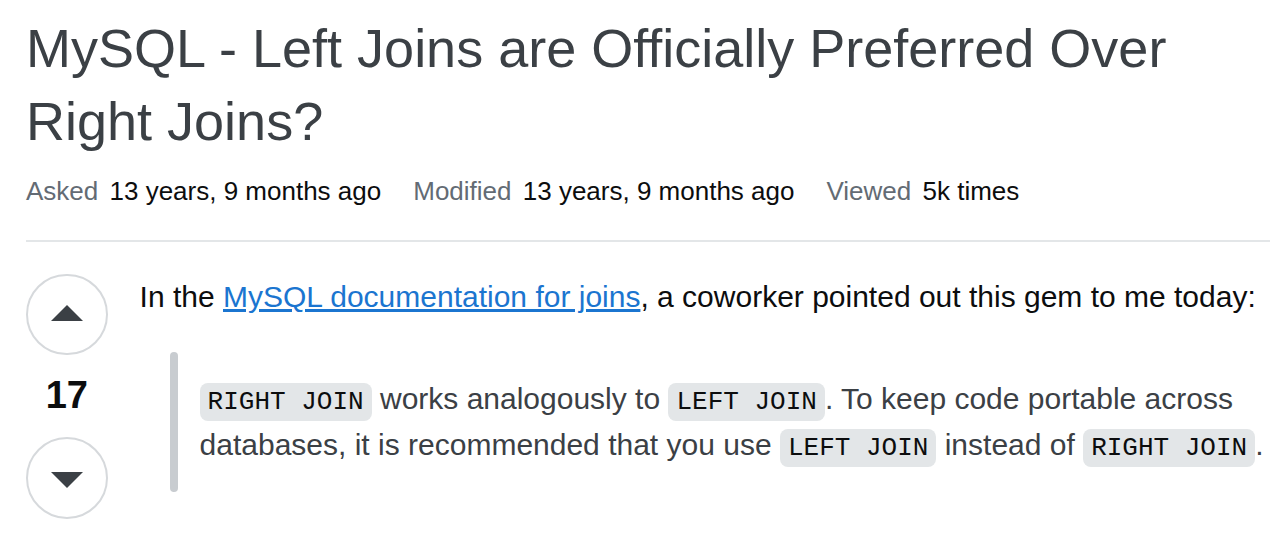
\includegraphics[width=0.45\textwidth]{mysql2.png}
    \end{center}
    \vspace{0.5em}
    \begin{itemize}
        \item Algumas documentações (como as do MySQL) indicam que o \texttt{RIGHT JOIN} é internamente convertido para um \texttt{LEFT JOIN} com a ordem das tabelas invertida.
        \item Isso explica por que, na prática, muitos desenvolvedores preferem usar apenas \texttt{LEFT JOIN} para padronizar o código.
    \end{itemize}
\end{frame}

% Slide Extra: Compatibilidade entre SGBDs
\begin{frame}{Compatibilidade: SQLite vs PostgreSQL}
    Nem todos os bancos de dados suportam todos os tipos de Join nativamente:
    \vspace{1em}
    \begin{columns}
        \begin{column}{0.45\textwidth}
            \begin{exampleblock}{SQLite}
                \textbf{Não implementa} o \texttt{RIGHT JOIN} nem o \texttt{FULL JOIN}. É necessário inverter as tabelas em um \texttt{LEFT JOIN} para obter o mesmo resultado.
            \end{exampleblock}
        \end{column}
        \begin{column}{0.45\textwidth}
            \begin{exampleblock}{PostgreSQL}
                \textbf{Implementação Completa}. Suporta nativamente \texttt{RIGHT JOIN} e \texttt{FULL JOIN}, seguindo fielmente o padrão SQL ANSI.
            \end{exampleblock}
        \end{column}
    \end{columns}
    \vspace{1em}
    \centering
    \small \textbf{Conclusão:} O \texttt{LEFT JOIN} é o mais universal.
\end{frame}

% Slide 8: FULL JOIN
\begin{frame}[fragile]{FULL OUTER JOIN (Tudo)}
    \begin{columns}
        \begin{column}{0.6\textwidth}
            Retorna \textbf{todos} os registros de ambas as tabelas, unindo onde houver correspondência.
            \begin{lstlisting}
SELECT A.nome, C.nome_curso
FROM Alunos AS A
FULL JOIN Cursos AS C ON A.curso_id = C.id;
            \end{lstlisting}
        \end{column}
        \begin{column}{0.35\textwidth}
            \centering
            \begin{tikzpicture}[scale=0.8]
                \fill[maincolor!60] (0,0) circle (1.2);
                \fill[maincolor!60] (1.2,0) circle (1.2);
                \draw (0,0) circle (1.2);
                \draw (1.2,0) circle (1.2);
                \node at (-0.5,0) {\scriptsize \textbf{Alunos}};
                \node at (1.7,0) {\scriptsize \textbf{Cursos}};
            \end{tikzpicture}
        \end{column}
    \end{columns}
    \textbf{Resultado:}
    \small
    \begin{table}
        \begin{tabular}{ll}
        \toprule
        \textbf{nome} & \textbf{nome\_curso} \\ \midrule
        Ana & Engenharia \\
        João & Direito \\
        \alert{Pedro} & \alert{NULL} \\
        \alert{NULL} & \alert{Medicina} \\ \bottomrule
        \end{tabular}
    \end{table}
\end{frame}

% Slide Extra: LEFT JOIN (Exclusivo)
\begin{frame}[fragile]{LEFT JOIN (Exclusivo)}
    \begin{columns}
        \begin{column}{0.6\textwidth}
            Retorna apenas os registros da esquerda que \textbf{não possuem par} na direita.
            \begin{lstlisting}
SELECT A.nome, C.nome_curso
FROM Alunos AS A
LEFT JOIN Cursos AS C ON A.curso_id = C.id
WHERE C.id IS NULL;
            \end{lstlisting}
        \end{column}
        \begin{column}{0.35\textwidth}
            \centering
            \begin{tikzpicture}[scale=0.8]
                \fill[maincolor!60] (0,0) circle (1.2);
                \begin{scope}
                    \clip (1.2,0) circle (1.2);
                    \fill[white] (0,0) circle (1.2);
                \end{scope}
                \draw (0,0) circle (1.2);
                \draw (1.2,0) circle (1.2);
                \node at (-0.5,0) {\scriptsize \textbf{Alunos}};
                \node at (1.7,0) {\scriptsize \textbf{Cursos}};
            \end{tikzpicture}
        \end{column}
    \end{columns}
    \textbf{Resultado:}
    \small
    \begin{table}
        \begin{tabular}{ll}
        \toprule
        \textbf{nome} & \textbf{nome\_curso} \\ \midrule
        \alert{Pedro} & \alert{NULL} \\ \bottomrule
        \end{tabular}
    \end{table}
\end{frame}

% Slide Extra: RIGHT JOIN (Exclusivo)
\begin{frame}[fragile]{RIGHT JOIN (Exclusivo)}
    \begin{columns}
        \begin{column}{0.6\textwidth}
            Retorna apenas os registros da direita que \textbf{não possuem par} na esquerda.
            \begin{lstlisting}
SELECT A.nome, C.nome_curso
FROM Alunos AS A
RIGHT JOIN Cursos AS C ON A.curso_id = C.id
WHERE A.id IS NULL;
            \end{lstlisting}
        \end{column}
        \begin{column}{0.35\textwidth}
            \centering
            \begin{tikzpicture}[scale=0.8]
                \fill[maincolor!60] (1.2,0) circle (1.2);
                \begin{scope}
                    \clip (0,0) circle (1.2);
                    \fill[white] (1.2,0) circle (1.2);
                \end{scope}
                \draw (0,0) circle (1.2);
                \draw (1.2,0) circle (1.2);
                \node at (-0.5,0) {\scriptsize \textbf{Alunos}};
                \node at (1.7,0) {\scriptsize \textbf{Cursos}};
            \end{tikzpicture}
        \end{column}
    \end{columns}
    \textbf{Resultado:}
    \small
    \begin{table}
        \begin{tabular}{ll}
        \toprule
        \textbf{nome} & \textbf{nome\_curso} \\ \midrule
        \alert{NULL} & \alert{Medicina} \\ \bottomrule
        \end{tabular}
    \end{table}
\end{frame}

% Slide Extra: FULL OUTER JOIN (Exclusivo)
\begin{frame}[fragile]{FULL OUTER JOIN (Exclusivo)}
    \begin{columns}
        \begin{column}{0.6\textwidth}
            Retorna tudo o que \textbf{não é comum} entre as duas tabelas.
            \begin{lstlisting}
SELECT A.nome, C.nome_curso
FROM Alunos AS A
FULL JOIN Cursos AS C ON A.curso_id = C.id
WHERE A.id IS NULL OR C.id IS NULL;
            \end{lstlisting}
        \end{column}
        \begin{column}{0.35\textwidth}
            \centering
            \begin{tikzpicture}[scale=0.8]
                \fill[maincolor!60] (0,0) circle (1.2);
                \fill[maincolor!60] (1.2,0) circle (1.2);
                \begin{scope}
                    \clip (0,0) circle (1.2);
                    \fill[white] (1.2,0) circle (1.2);
                \end{scope}
                \draw (0,0) circle (1.2);
                \draw (1.2,0) circle (1.2);
                \node at (-0.5,0) {\scriptsize \textbf{Alunos}};
                \node at (1.7,0) {\scriptsize \textbf{Cursos}};
            \end{tikzpicture}
        \end{column}
    \end{columns}
    \textbf{Resultado:}
    \small
    \begin{table}
        \begin{tabular}{ll}
        \toprule
        \textbf{nome} & \textbf{nome\_curso} \\ \midrule
        \alert{Pedro} & \alert{NULL} \\
        \alert{NULL} & \alert{Medicina} \\ \bottomrule
        \end{tabular}
    \end{table}
\end{frame}

% Slide 9: CROSS JOIN
\begin{frame}[fragile]{CROSS JOIN (Produto Cartesiano)}
    Combina \textbf{cada linha} da primeira tabela com \textbf{todas as linhas} da segunda.
    \begin{lstlisting}
SELECT A.nome, C.nome_curso FROM Alunos AS A
CROSS JOIN Cursos AS C;
    \end{lstlisting}
    \textbf{Resultado (9 linhas):}
    \small
    \begin{center}
    \begin{tabular}{ll}
    \toprule
    Ana & Engenharia \\
    Ana & Direito \\
    Ana & Medicina \\
    João & Engenharia... (continua) \\ \bottomrule
    \end{tabular}
    \end{center}
\end{frame}

% Slide 10: Resumo
\begin{frame}{Resumo para não esquecer}
    \begin{itemize}
        \item \textbf{INNER JOIN}: O que elas têm em comum.
        \item \textbf{LEFT JOIN}: Tudo da esquerda + o que houver na direita.
        \item \textbf{RIGHT JOIN}: Tudo da direita + o que houver na esquerda.
        \item \textbf{FULL JOIN}: A união completa (mesmo sem par).
        \item \textbf{CROSS JOIN}: Todas as combinações possíveis.
    \end{itemize}
    \vspace{1em}
    \centering
    \textbf{Dúvidas?}
\end{frame}

\end{document}
